\subsection{Thresholding / Binarization}
    Pixels with intensity \textit{below} threshold $\rightarrow$ black\\
    Pixels with intensity \textit{above} threshold $\rightarrow$ white\\
    \textbf{Threshold} usually between fore- and background peak.
    
    \subsubsection{Adaptive Thresholding}
        Compute threshold seperately for smaller regions.\\
        (useful if multiple objects present)  

    \subsubsection{Dilation/ Erosion}
        After Thresholding, regions can be distorted by noise and texture.
        \begin{description}
            \item[Dilation:] Bright regions grow
            \item[Erosion:] Bright regions shrink
        \end{description}
        \begin{center}
            \resizebox{\linewidth}{!}{
               \includegraphics[
                    page = {5},
                    trim = {5.8cm, 2.2cm, 5.8cm, 11.3cm},
                    clip
                ]{Computer_Vision/08_2020-11-24_ComputerVision.pdf}
            }
        \end{center}
    \vfill \null \columnbreak

\subsection{Histogram Equalization}
    Increase global contrast, create flat histogram.\\ (Spread intensities to whole spectrum)\\
    \begin{minipage}{0.45\linewidth}
        \resizebox{\linewidth}{!}{
           \fbox{ \includegraphics[
                page = {3},
                trim = {7cm, 4cm, 21.7cm, 5cm},
                clip
            ]{Computer_Vision/08_2020-11-24_ComputerVision.pdf}
        }}
    \end{minipage}
    $\rightarrow$
    \begin{minipage}{0.44\linewidth}
        \resizebox{\linewidth}{!}{
           \fbox{ \includegraphics[
                page = {3},
                trim = {17.7cm, 4.05cm, 11.2cm, 5.05cm},
                clip
            ]{Computer_Vision/08_2020-11-24_ComputerVision.pdf}
        }}
    \end{minipage}

\subsection{Image Filtering}
    Replace pixel value with:
    \begin{description}
        \item[Mean:]  \textit{mean} of neighbouring pixels.
        \item[Gaussian:]  \textit{weighted mean} of neighbouring pixels.
        \item[Median:]  \textit{median intensity} in the window. (sorting)
    \end{description}
     
    \hfill
    \begin{minipage}{0.4\linewidth}
        \textbf{Mean Filter:}\\[0.5em]
        \begin{TAB}(@,4mm,4mm){c}{ccc}
            \phantom{.} \\
            $\frac{1}{9}$\\
            \phantom{.}
        \end{TAB}
        \begin{TAB}(e,4mm,4mm){|c|c|c|}{|c|c|c|}
            1 & 1 & 1 \\
            1 & 1 & 1 \\
            1 & 1 & 1   
        \end{TAB}
    \end{minipage}
    \begin{minipage}{0.5\linewidth}
        \textbf{Gaussian Filter:}\\[0.5em]
        \begin{TAB}(@,4mm,4mm){c}{ccc}
            \phantom{.} \\
            $\frac{1}{16}$\\
            \phantom{.}
        \end{TAB}
        \begin{TAB}(e,4mm,4mm){|c|c|c|}{|c|c|c|}
            1 & 2 & 1 \\
            2 & 4 & 2 \\
            1 & 2 & 1   
        \end{TAB}
    \end{minipage}
    \subsection{Edge Detection}
        \subsubsection{Canny Edge Detector}
            \begin{enumerate}
                \item Gaussian Filter to remove noise
                \item Find Gradient, Edge Strength and Orientation
                \item Non-Maxima Suppression
                \item Hysteresis Thresholding
            \end{enumerate}
            \subsubsubsection{Hysteresis Thresholding}
                \begin{enumerate}
                    \item Start with Gradient and Direction Map, compare neighbours along edge direction $\rightarrow$ Non-Maxima Suppression map
                    \item Mark values above $T_H$ (strong edge), set values below $T_L$ to zero (weak edge)
                    \item Compare neighbors along edge direction; if neighbour to strong edge is above $T_L$ $\rightarrow$ strong edge
                    \item Repeat 3. ("Chain reaction")
                \end{enumerate}
            \vfill \null \columnbreak
        \subsection{Hough Transform}
            Feature Extraction technique
            \begin{enumerate}
                \item Use normal representation of line:
                    $$
                        x \cos(\theta) + y \sin(\theta) = \rho
                    $$
                \item For each edge point $(x,y)$, plot normal representation for all $\theta$ $\rightarrow$ Hough Space
                \item Intensities in Hough plot accumulate\\
                        $\rightarrow$ overlapping points get brighter; peak values describe lines in the image 
                \item Extract $(\rho, \theta)$ of points with higher intensities
            \end{enumerate}
